\chapter[Revisão de Literatura]{Revisão de Literatura}

%\addcontentsline{toc}{chapter}{Revisão de Literatura}
% ----------------------------------------------------------

Nesse capítulo é feita uma revisão no estado da arte dos algoritmos de roteamento de veículos a aplicação de algoritmos genéticos para mesma finalidade.

\section{Roteamento de Veículos com Janelas de Tempo}

O PRVJT é amplamente estudado na literatura de pesquisa operacional. Tendo pelo menos duas frentes de soluções, as exatas e as baseadas em heurísticas. 


\subsection{Formulação matemática}

O PRVJT pode ser definido a partir um grafo completo orientado~\(G = (V,A)\) em que \(V = {0,\cdots,n+1}\) é um conjunto de vértices e \(G ={(i,j)|i,j \in V}\) é o conjunto de arcos.
Cada arco (i,j) é associado a um tempo \(t_{ij}\) e um custo de travessia \(c_{ij}\).

É necessário uma definição precisa do termo \textit{custo de travessia}. Em casos práticos pode se considerar diversos fatores, tais como distancia, tempo, desgaste do veículo ao percorrer determinado caminho, entre outros fatores. Porém, quando se trata de problemas teóricos envolvendo janelas de tempo, é comum converter todas as medidas relevantes em unidades de tempo para fins de padronização e também para facilitar a comparação entre diferentes métodos. Por isso, adota-se aqui a mesma definição de custo que a maioria dos trabalhos teóricos da literatura, considerando que o custo de viagem consiste na distância convertida em unidades de tempo. \cite{ROCHAT}

Podemos descrever o problema como sendo um conjunto \(K\) de veículos com capacidade \(Q\), eles devem atender \(n\) clientes, representados pelos vértices \(1,\cdots,n\). Considera-se que \(N = V \{0, n + 1\}\) representa o conjunto de clientes. Os veículos devem partir do depósito e, após visitar todos os clientes, devem retornar ao mesmo local de onde partiram. Por conveniência, o deposito é representado por dois vértices, o vértice \(0\), que representa a origem, e o vértice \(n+1\) que representa o destino. A cada cliente \(i\), uma demanda \(q_i\) é associada, esta deve ser atendida por um único veículo. E todos os vértices possuem uma janela de tempo \([e_i,l_i]\), o serviço no vértice \(i\) deve ser iniciado dentro desse intervalo. Caso ocorra que a chegada ao cliente \(i\) aconteça antes do horário previsto \(e_i\), ele deve esperar a abertura da janela. O veículo não poderá chegar a \(i\) depois do instante \(l_i\), pois isso faria violar a restrição de tempo do problema. Esse tipo de restrição é conhecido na literatura como janela de tempo rígida. A cada vértice é também associado um tempo de serviço, denotado por \(s_i\). O objetivo é encontrar uma solução \(s\) de custo mínimo, de forma a minimizar a soma de todos os custos de viagem \(\sum_{(i,j) \in s} c_{ij}\) que são associados aos arcos \((i,j)\) presentes nas rotas que compõem essa solução.

A formulação matemática do PRVJT, é apresentada pelas expressões:

\begin{equation}  \label{eq:prvjt1}
\min
 \sum_{k \in K}\sum_{i \in V}\sum_{j \in V} c_{ij}x_{ijk}
\end{equation}

Sujeito às seguintes restrições:

\begin{equation} \label{eq:prvjt2}
\sum_{k \in K}\sum_{j \in V} x_{ijk} = 1, \forall i \in N
\end{equation}

\begin{equation} \label{eq:prvjt3}
\sum_{j \in V} x_{0jk} = 1, \forall k \in K
\end{equation}

\begin{equation} \label{eq:prvjt4}
\sum_{i \in V} x_{ijk} - \sum_{i \in V} x_{jik} = 0, \forall k \in K, \forall j \in N
\end{equation}

\begin{equation} \label{eq:prvjt5}
\sum_{i \in V} x_{i(n+1)k} = 1, \forall k \in K
\end{equation}

\begin{equation} \label{eq:prvjt6}
\sum_{i \in N} q_i \sum_{j \in V} x_{ijk} \leq Q, \forall k \in K
\end{equation}

\begin{equation} \label{eq:prvjt7}
b_{ik} + s_i + t_{ij} -(1-x_{ijk})M_{ij} \leq b_{jk},\forall k \in K, \forall (i,j) \in A
\end{equation}

\begin{equation} \label{eq:prvjt8}
e_i \leq b_{ik} \leq l_i,\forall k \in K,\forall i \in V
\end{equation}

\begin{equation} \label{eq:prvjt9}
x_{ijk} \in \{0,1\},\forall k \in K,\forall (i,j) \in A
\end{equation}

A variável binária \(x_{ijk}\) assume valor 1 se o veículo \(k\) passa pelo arco (i,j) e 0, caso contrário.

A função objetivo \ref{eq:prvjt1} expressa o custo total a ser minimizado. 
As restrições \ref{eq:prvjt2} asseguram que somente um veículo \(k\) sai de cada cliente \(i\). 
As restrições \ref{eq:prvjt3}, \ref{eq:prvjt4}, \ref{eq:prvjt5} garantem a continuidade do caminho a ser percorrido pelo veículo \(k\), ou seja, cada veículo parte do depósito, visita os clientes e em seguida retorna ao depósito. 
As restrições \ref{eq:prvjt6} fazem com que cada veículo \(k\) somente possa atender a um conjunto de clientes cuja demanda total não ultrapasse sua capacidade Q. 
As restrições \ref{eq:prvjt7}, \ref{eq:prvjt8} asseguram a viabilidade das rotas no que diz respeito as restrições de janelas de tempo, em que \(b_{ik}\) representa o tempo em que o veículo \(k\) começa a atender o cliente \(i\) e \(M_{ij}\) são constantes de valor suficientemente grande.  As restrições \ref{eq:prvjt9} definem o domínio das variáveis de decisão.~\cite{CORDEAU}


\subsection{Complexidade}

Encontrar a solução ótima do PRVJT implica em obter simultaneamente a solução de vários problemas NP-difíceis, dentre os quais citam-se o \textit{Problema do Caixeiro Viajante} (PCV) e o \textit{Problema da Mochila}. Sendo assim, tal tarefa é também NP-difícil. Além disso, encontrar uma simples solução viável para o PRVJT dispondo de um conjunto limitado de veículos é NP-difícil no sentido forte \cite{Kohl}. Porém, uma solução inicial viável é trivial caso o número de veículos seja ilimitado, bastando atender cada consumidor com um veículo.

Os atuais resultados encontrados na literatura referentes ao PRVJT comprovam que os algoritmos exatos restringem-se à resolução de problemas-teste com tamanho reduzido e janelas de tempo apertadas. Embora hoje podemos resolver problemas com um tamanho que seja ligeiramente maior que o de alguns anos atrás, o crescimento da capacidade dos computadores e da eficiência dos algoritmos esta muito distante da curva exponencial representada por este problema. Pode-se dizer que os métodos exatos não são uma alternativa viável para situações onde a um número maior de consumidores, como ocorre na maioria dos casos reais. \cite{Chabrier}

Abordagens heurísticas e algoritmos aproximativos também tem sido utilizadas na resolução do PRVJT. As Heurísticas buscam obter uma solução em tempo hábil. Este fato torna as estratégias heurísticas muito poderosas se comparadas com abordagens exatas, que focam exclusivamente na obtenção da solução ótima. Uma boa heurística deve ser capaz de encontrar soluções próximas da ótima, em tempo bem inferior ao necessário pelos métodos exatos. A qualidade da solução não deve variar demasiadamente ao aplicá-la em diferentes ou ao mesmo problemas-teste. Até 2006, 45 do total de 56 problemas de Solomon tiveram uma solução ótima. Alguns casos foram gastos mais que cinco horas de processamento na resolução de algumas instancias, enquanto em outras puderam ser resolvidas em menos de um minuto. ~\cite{Jepsen}

Os métodos aproximativos vem ao encontro destas características. Um método aproximativo é uma heurística com garantia de qualidade no resultado. A melhor solução encontrada por um algoritmo de aproximação esta sempre a uma distancia percentual previamente definida da solução ótima desconhecida. A "distancia do ótimo" é particular de cada algoritmo, podendo até não ser muito relevante em termos práticos. Um exemplo bem conhecido é o algoritmo PRIM, para árvore geradora mínima, que é capaz de oferecer uma solução viável para o PCV, que é no máximo duas vezes o ótimo em distância total percorrida \cite{Alvarenga}.

Dado essa complexidade, resolver esse problema utilizando de abordagens puramente exatas é uma tarefa extremamente árdua, demandando tempo computacional muito elevado. Por isso é motivado o desenvolvimento de novos algoritmos heurísticos com tempos mais reduzidos para a solução do PRVJT, mesmo que esses não garantam uma solução ótima.

\subsection{Heurísticas}

Heurísticas são procedimentos de busca que visam a obtenção de soluções com uma qualidade satisfatória em um tempo computacional aceitável. Porem tais procedimentos não garantem encontrar a solução ótima nem são capazes de mensurar o quão próxima a solução obtida está da ótima. Será exemplificada as ideias centrais de algumas heurísticas construtivas e de refinamento disponíveis na literatura.

\subsubsection{Construção de rotas}

Um dos trabalhos mais antigos sobre heurística para construção de rotas para PRVJT proposto por Baker \cite{Baker} em 1989, Foi criada a partir da ideia da heurística das economias de Clarke e Write \cite{Clarke} que foi proposta para criação de soluções para o PRV. O algoritmo funciona primeiramente criando uma rota partindo do depósito para cada cliente \textit{i}, para em seguida, executar varias vezes, em cada vez, o algoritmo calcula quais duas rotas que podem ser combinadas de forma a gerar a maior economia possível.

Outra heurística proposta por \cite{VANLANDEGHEM} também baseada na heurística das economias é uma heurística de dois critérios, nesta as janelas de tempo são utilizadas para mensurar o quanto uma ligação entre dois clientes é boa em termos de tempo.

De forma semelhante \cite{Solomon} desenvolveu um algoritmo baseado na ideia na heurística das economias para resolução do PRVJT. Devido a existência de janelas de tempo, deve-se considerar também a orientação da rora. Também deve-se checar as violações de janelas de tempo quando mais de uma rota é combinada. Ela de forma igual a heurística das Economias original possuem complexidade \(O^2 log n^2\).
Nesta heurística toda rota é inicializada encontrando o cliente mais próximo ao depósito que ainda não pertença a nenhuma rota. A cada iteração subsequente o cliente mais próximo ao último adicionado à rota é considerado para inserção ao final da rota que está sendo gerado. Quando a busca falha, uma nova rota é inicializada.

As heurísticas de \cite{VANLANDEGHEM} e \cite{Solomon} de forma geral conseguem encontrar uma solução rapidamente. Porém as soluções que suas heurísticas encontram são geralmente de baixa qualidade. Geralmente pouco a mais de 10\% do ótimo ~\cite{Sherbeny}.

Criar uma rota por vez traz uma desvantagem, usualmente as rotas geradas por último são de baixa qualidade, uma vez que os clientes sem rota tendem estar distantes geograficamente~\cite{Sherbeny}. 

É possível encontrar uma tentativa de solução deste problema de inserção no trabalho de Rousseau~\cite{Rousseau} por meio de construção simultânea de varias rotas. A inicialização das rotas é feita usando a heurística de inserção de Solomon. Em cada rota o cliente mais distante do depósito é selecionado como semente.  A partir desse ponto, computa-se a melhor inserção viável para cada cliente que ainda não foi visitado. Este método é melhor que a heurística de Solomon, porem as soluções geradas continuam distantes das ótimas.

Antes e Derigs \cite{Derigs} evoluem as ideias clássicas de inserção. No seu trabalho, todo cliente sem rota designada recebe um custo de inserção de cada uma das rotas. A definição desse custo é semelhante ao adotado nas  heurísticas de Solomon.  Cada cliente sem rota envia uma proposta a rota com melhor oferta, cada rota aceita a melhor proposta dos clientes com menor número de alternativas.  Vale observar que mais clientes podem ser inseridos em cada iteração.  Se houver alguma violação nas rotas,  um certo numero de veículos é removido e o processo é reiniciado. 

Os resultados do trabalhos de Antes e Derigs \cite{Derigs} são comparados aqueles apresentados por Potvin e Rousseau~\cite{Rousseau}. Segundo os autores, construir rotas paralelamente produz soluções de maior qualidade que construir rotas uma a uma.


\subsubsection{Aprimoramento de rotas}

Quase todas as heurísticas de melhoria de rotas tem a noção de vizinhança. A vizinhança de uma solução S é um conjunto de soluções N(s) que podem ser geradas pela aplicação de uma única alteração denominada \textit{movimento} na solução S.

Checar algumas ou todas as soluções de uma vizinhança pode revelar soluções melhores em relação a uma determinada função objetivo. Esta ideia pode ser repetida partindo-se da melhor solução obtida até o momento. Se em algum momento nenhuma solução melhor for encontrada em uma vizinhança, um ótimo local foi obtido.  Trata-se definitivamente de um ótimo local, porem este pode eventualmente ser um ótimo global.  A este algoritmo da-se o nome de Hill Climbing.~\cite{Gendreau}.
Na próxima seção serão introduzidas varias estruturas de vizinhança empregadas na literatura para melhorar soluções do PRVJT. Em seguida serão descritos alguns dos algoritmos que as utilizam.

\subsubsection{Estruturas de vizinhança}

Uma estrutura de vizinhança mais utilizada em roteamento é a \textit{k-opt}, onde \textit{k} arcos são removidos e substituídos por outros \textit{k} arcos. Um ótimo local obtido utilizando-se a vizinhança \textit{k-opt} é dita solução \textit{k-optimal}. Normalmente, k é no máximo 3.

Para todas as possíveis trocas \textit{2-opt} e algumas das permutações da vizinhança \textit{3-opt}, parte da rota é invertida. Isto comumente acarreta violações nas janelas de tempo. No trabalho de \cite{Potvin} são apresentadas duas variantes, a \textit{2-opt*}  e a \textit{Or-opt}, que mantêm a direção da rota.

Na vizinhança \textit{Or-opt}, um conjunto contíguo de até 3 clientes é realocado para outra posição na mesma rota. Uma vez que nessa vizinhança três arcos são trocados por outros três, é fácil observar que ela é um subconjunto da vizinhança \textit{3-opt}. Desta forma, o tamanho da vizinhança é reduzido de O(\(n^3\)) para O(\(n^2\). De forma geral, o tamanho da vizinhança \textit{k-opt}  é da ordem de O(\(n^k\)). A vizinhança 2-opt* consiste na troca de um
segmento de uma rota por um segmento de outra rota. Esses operadores de vizinhança são muitas vezes denotados na literatura por \textit{crossover} ou simplesmente \textit{cross}.

Movimentos da vizinhança \textit{exchange} alteram diferentes rotas através da troca simultânea
de dois clientes. A vizinhança k-node, proposta no trabalho de \cite{Christofides} tem sido adaptada por alguns autores para que este leve em consideração aspectos referentes às janelas de tempo. Nesta estrutura, cada cliente i é considerado e os conjuntos M1 e M2 são identificados. Em M1 são alocados o cliente i e seu sucessor j. O conjunto M2 é formado pelos clientes mais próximos aos clientes i e j que não estejam na mesma rota que i e j (encontrados pela minimização do custo de inserção considerando distância euclidiana). A vizinhança é então definida pela remoção dos elementos desses conjuntos e posterior inserção em qualquer outra possível localização. Como trata-se de uma vizinhança de dimensões muito elevadas, apenas os k candidatos mais promissores são considerados. 

Outra vizinhança explorada na literatura é a \(\lambda-interchange\) desenvolvida em \cite{Osman}, originalmente para o PRV. Trata-se de uma generalização do operador \textit{relocate}. Nesta estrutura, um subconjunto de clientes de uma mesma rota é trocado por outro conjunto de outra rota. O mecanismo de geração \(\lambda-interchange\) pode ser descrito como segue. Dada uma solução para o problema, representada pelo conjunto de rotas \(S = \{r_1, \cdots,r_p, \cdots,r_q,\cdots,r_k\}\), um \(\lambda-interchange\) entre um par de rotas \((r_p, r_q)\) consiste na troca dos clientes \(S_1\bigcup r_p\) de tamanho \(|S_1|\leq\lambda\) por outro subconjunto \(S_2\bigcup r_q\) de tamanho \(|S_2|\leq\lambda\) para gerar novas rotas \(r^\ast_p = (r_p-S_1)\bigcup S_2, r^\ast_p = (r_q - S_2) \bigcup S_1 \) e uma nova solução  \(S' = \{r_1, \cdots,r^\ast_p, \cdots,r^\ast_q,\cdots,r_k\}\).
A vizinhança \(N_\lambda(S)\) de uma dada solução S é o conjunto de todos os vizinhos S' gerados para um dado valor de \(\lambda\).

A vizinhança denotada por \textit{shift-sequence} é proposta em \cite{Schulze}.  Nesta, um cliente é movido de uma rota para outra checando-se todas as possibilidades de inserção. Caso uma inserção possa se tornar viável pela remoção de outro cliente j, este é removido e inserido em outra rota. Este procedimento é repetido até que a viabilidade seja restabelecida.

A Tabela \ref{table:vizinhanca} apresenta uma breve descrição das estruturas de vizinhança comumente
utilizadas na literatura por algoritmos de busca local para a resolução do PRVJT. Observa-se
que algumas dessas são também utilizadas neste trabalho

\newcolumntype{C}[1]{>{\centering\let\newline\\\arraybackslash\hspace{0pt}}m{#1}}
\begin{table}[h] 
	\centering
	\vspace{0.5cm}
	\renewcommand{\arraystretch}{2.0}
	\caption{Estruturas de vizinhança para o PRVJT}
	\label{table:vizinhanca}
	\begin{tabular}{|C{4cm}|C{11cm}|}
		\hline
		\textbf{Vizinhança} & \textbf{Descrição} \\
		\hline
		\textit{Relocate} & Move um cliente de uma rota para outra.  \\
		\hline
		\textit{Exchange} & Troca dois clientes entre duas rotas  \\
		\hline
		\(2-opt^\ast\) & Troca um segmento de uma rota por um segmento de outra rota.  \\
		\hline
		\textit{Or-opt} & Um segmento contínuo de clientes é movido de uma posição em uma rota para outra posição da mesma rota. \\
		\hline
		\textit{k-node} & Os clientes \(i\), seu sucessor \(j\) e os dois clientes mais próximos que não estão na mesma rota são removidos. Tenta-se então inserir os quatro vértices em todas as possíveis localizações. Como trata-se de uma vizinhança de dimensões muito elevadas, apenas os k candidatos mais promissores são considerados.\\
		\hline
		\(\lambda-interchange\) & Um subconjunto \(S_1\) de clientes de tamanho \(|S_1|\leq \lambda\) de uma rota é
		trocado por um subconjunto \(S_2\) de tamanho \(|S_2| \leq \lambda\) de outra rota.
  \\
		\hline		
		\textit{Shift-sequence} & Um cliente é movido de uma rota para outra checando-se todas as possibilidades de inserção. Caso uma inserção se torne viável pela remoção de um consumidor \(j\), este é removido e inserido em alguma outra rota. Este procedimento é repetido até que a viabilidade seja restabelecida. \\
		\hline
	\end{tabular}
\end{table} 

\subsection{Meta-heurísticas}

Meta-heurísticas são procedimentos destinados a encontrar uma boa solução, eventualmente a ótima, consistindo na aplicação, em cada passo, de uma heurística subordinada, a qual tem que ser modelada para cada problema específico \cite{Ribeiro} Contrariamente às heurísticas convencionais, as metaheurísticas são de caráter geral e providas de mecanismos para tentar escapar de ótimos locais. \cite{Souza}

\subsubsection{Busca Tabu (Tabu Search)}

Essa meta-heurística foi introduzida por \cite{Glover}, mas foi \cite{Garcia} propos a primeira aplicação para o problema de roteamento e programação de veículos com janela de tempo. O conceito básico da busca tabu (BT) é explorar o espaço solução, a cada iteração, movendo de uma dada solução para outra que pertença à sua vizinhança. Diferentemente dos métodos clássicos de descida, aceita-se soluções piores, o que pode gerar ciclos. Para evitar a ciclagem, as soluções já avaliadas são marcadas como proibidas e incluídas em uma lista tabu.

\subsubsection{Têmpera Simulada (Simulated Annealing)}

A têmpera simulada (TS) é uma técnica de relaxação estocástica baseada no processo térmico utilizado na metalurgia para obtenção de estados de baixa energia num sólido.  No algoritmo da TS,  uma nova solução \(x_t\) é aceita sempre que \(f(xt) < f(x)\), onde x é a solução corrente. Para fugir dos mínimos locais, soluções com \(f(x_t) \geq f(x)\) também são aceitas com uma probabilidade \(e^{\delta/T}\), onde \(\delta = f(x_t) - f(x)\) e T é um parâmetro (chamado temperatura) que varia ao longo das iterações, partindo de um número grande e terminando próximo de zero. A queda na temperatura ocorre gradativamente e costuma ser feita através da regra  \(T_k = \alpha T_(k-1)\) para \(0 \leq \alpha \leq 1\). \cite{Russell}

\subsubsection{Busca Local com Múltiplos Pontos Iniciais (Multi-Start Local Search)}

Este método de busca local envolve a geração de um conjunto de soluções iniciais, seguida da aplicação de um procedimento de refinamento a cada solução gerada. As diferentes soluções iniciais permitem uma diversificação do espaço de busca, o que evita ótimos locais. A heurística de inserção mais barata é usada para criar a solução inicial, que é refinada por uma extensão da heurística de cadeia de ejeções, com o objetivo de reduzir o número de veículos. Finalmente, uma modificação da troca cruzada é empregada para reduzir a distância total percorrida em cada solução. \cite{Dullaert}

\subsubsection{Algoritmos Genéticos / Evolutivos}

Algoritmos genéticos e evolutivos são meta-heurística com boas aplicações no problema de PRV e PRVJT, \cite{Homberger}  propuseram duas estratégias evolucionárias diferentes. As duas estratégias utilizam uma aproximação estocástica baseada na heurística das economias, ou seja, os clientes pertencentes a lista das economias são escolhidos aleatoriamente para constituir a rota. A função objetivo pondera o número de rotas, a distância total e um critério que determina a facilidade de eliminação da menor rota. A mutação é feita pelas heurísticas de refinamento \textit{Or-opt}, \({2-opt\ast}\) e \(\lambda-Interchange\). No primeiro algoritmo, o cruzamento não é executado. No segundo, o cruzamento é feito através de um procedimento uniforme.

Foi desenvolvido por \cite{Jung} um algoritmo genético híbrido, no qual a função objetivo é baseada na distância. O algoritmo começa com a aplicação da heurística de inserção de \cite{Solomon} para a determinação de uma solução inicial. O primeiro cliente de cada rota é escolhido de forma aleatória entre o cliente mais distante do depósito, o cliente com o menor instante final da janela de tempo e um cliente também determinado aleatoriamente. 

 Em seu algoritmo a seleção é feita pelo torneio. Para o cruzamento, o grafo que contém o depósito, os clientes e as arestas utilizadas para formar as rotas de cada veículo são mapeados e a escolha dos pontos de corte é feita por meio de curvas ou figuras geométricas de diferentes tipos A figura \ref{fig:jung} exemplifica o procedimento de cruzamento. As regiões formadas pela sobreposição das figuras geométricas definem conjuntos de nós. Cada conjunto pertence a um único pai. Primeiramente, definimos as rotas dentro desses conjuntos. Como essa divisão de nós é arbitrária, restarão várias rotas desconexas, de modo que é preciso utilizar algoritmos de reparação para reconstruir uma solução factível. Essa reconstrução é feita seguindo a regra do vizinho mais próximo.
 
 Na mutação, são feitas mudanças de nós entre, no máximo, 3 rotas. As heurísticas de refinamento \textit{or-opt}, \textit{relocate} são aplicadas ao final da iteração para melhorar a solução.  
 
 Algoritmos evolucionários para o problema com janela de tempo foram analisados e comparados por Braysy \cite{BraysyAG}.
 
\begin{minipage}{\linewidth}
	\makebox[\linewidth]{
		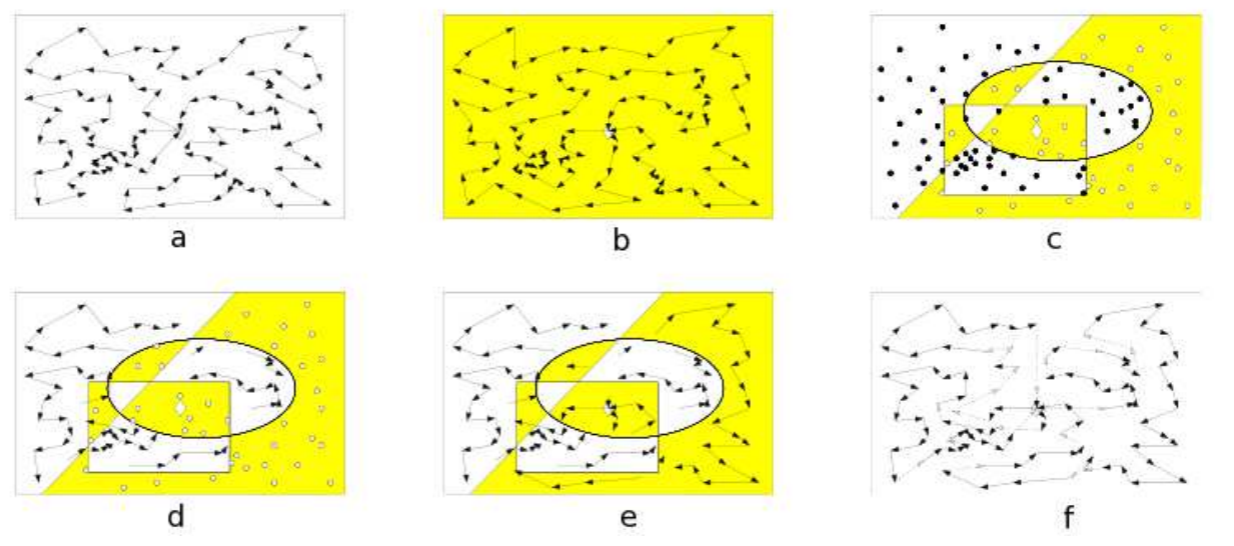
\includegraphics[keepaspectratio=true,scale=0.45]{ibagens/jung.png}}
	\captionof{figure}{O crossover utilizado por Jung e Moon. As Figuras a e b representam, respectivamente, os pais 1 e 2. A Figura c mostra a divisão dos clientes com base em figuras geométricas.  A Figura d mostra as ligações feitas nas regiões referentes ao primeiro pai, enquanto a Figura e mostra as rotas internas à região referente ao segundo pai. Finalmente, a Figura f mostra as rotas após a aplicação do algoritmo de reparação.
	 }
	\label{fig:jung}
\end{minipage}

% https://en.wikibooks.org/wiki/LaTeX/Mathematics
\section{Algoritmos genéticos}

AG é uma técnica amplamente utilizada de IA, que utilizam conceitos provenientes do princípio de seleção natural para abordar uma  ampla série de problemas, geralmente de adaptação. \cite{DiogoCLucas}

\subsection{Funcionamento}
 
Inspirado na maneira como o seleção natural explica o processo de evolução das espécies, Holland \cite{Holland1975} decompôs o funcionamento dos AG em sete etapas, essa são \textit{inicialização}, \textit{avaliação}, \textit{seleção}, \textit{cruzamento}, \textit{mutação}, \textit{atualização} e  \textit{finalização} conforme a Figura \ref{fig:EstruturaAG}. 

\begin{minipage}{\linewidth}
    \makebox[\linewidth]{
        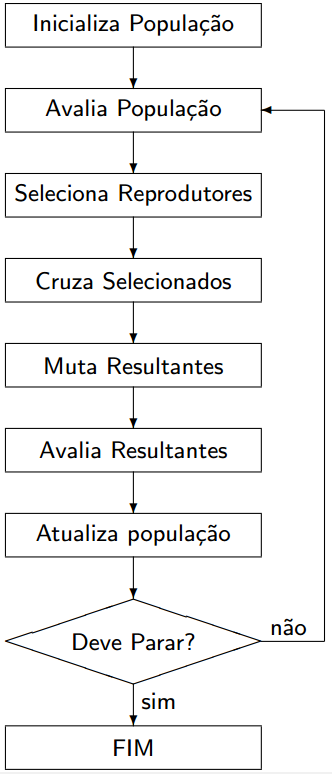
\includegraphics[keepaspectratio=true,scale=0.45]{ibagens/genetico1.png}}
    \captionof{figure}{Estrutura de um AG \cite{DiogoCLucas} }
    \label{fig:EstruturaAG}
\end{minipage}


\subsection{Inicialização}
Criar uma população de possíveis respostas para um problema. 
É comum fazer uso de funções aleatórias para gerar os indivíduos, sendo este um recurso simples que visa fornecer maior diversidade.

\subsection{Avaliação}
Avalia-se a aptidão das soluções, os indivíduos da população, então é feita uma análise para que se estabeleça quão bem elas respondem ao problema proposto.
A função de avaliação também pode ser chamada de função objetivo. Ela pode variar de acordo com problema,  
Calcular com exatidão completa o grau de adaptação dos indivíduos pode ser uma tarefa complexa em muitos casos, e se levarmos em conta que esta operação é repetida varias vezes ao longo do processo de evolução, seu custo pode ser consideravelmente alto. Em tais situações é comum o uso de funções não determinísticas, que não avaliam a totalidade das características do indivíduo, operando apenas sobre uma amostragem destas.

\subsection{Seleção}
Ela é a responsável pela perpetuação de boas características na espécie. 
Neste estágio que os indivíduos são escolhidos para posterior cruzamento, fazendo uso do grau de adaptação de cada um é realizado um sorteio, onde os indivíduos com maior grau de adaptação tem maior probabilidade de se reproduzirem.
O grau adaptação é calculado a partir da função de avaliação para cada individuo, determina o quão apto ele esta para reprodução relativo a sua população. 


\subsection{Cruzamento}
Após alguns indivíduos serem selecionados, normalmente pares, estes são usados como base para novos descendentes, combinando as suas características para gerar um novo genoma.

\subsection{Mutação}
Características dos indivíduos resultantes do processo de reprodução são alteradas, acrescentando assim variedade a população.
A mutação opera sobre os indivíduos resultantes do processo de cruzamento e com uma probabilidade pré-determinada efetua algum tipo de alteração em sua  estrutura. A importância desta operação é o fato de que uma vez bem escolhido seu modo de atuar, é garantido que diversas alternativas serão exploradas.


\subsection{Finalização}
É testado se as condições de encerramento da evolução foram atingidas, retornando para a etapa de avaliação em caso negativo e encerrando a execução em caso positivo.

Os critérios para a parada podem ser vários, desde o número de gerações criadas até o grau de convergência da população atual.

Toda base dos AG se fundamenta nos indivíduos, eles são a unidade básica em qual o algoritmo se baseia, sua função é codificar as possíveis soluções do problema a ser tratado e partir de sua manipulação no processo evolutivo, a partir daí que são encontradas as respostas.

Esses indivíduos precisam de uma representação, essa será o principal responsável pelo desempenho do programa. É comum chamar de \textit{genoma} ou \textit{cromossomo} para se referir ao individuo. Por essa definição podemos resumir um indivíduo pelos genes que possui, ou seja seu \textit{genótipo}.

Apesar de toda representação por parte do algoritmo ser baseada única e exclusivamente em seu genótipo, toda avaliação é baseada em seu fenótipo, o conjunto de características observáveis no objeto resultante do processo de decodificação dos genes do individuo, ver  Tabela \ref{table:genotipos}.

\newcolumntype{C}[1]{>{\centering\let\newline\\\arraybackslash\hspace{0pt}}m{#1}}
\begin{table}[h] 
    \centering
\vspace{0.5cm}
\renewcommand{\arraystretch}{2.0}
\caption{Exemplos de genótipos e fenótipos correspondentes em alguns tipos de problemas \cite{DiogoCLucas}}
\label{table:genotipos}
    \begin{tabular}{|C{4cm}|C{3.5cm}|C{7cm}|}
        \hline
        \textbf{Problema} & \textbf{Genótipo} & \textbf{ Fenótipo} \\
        \hline                  
        Otimização numérica & 0010101001110101 & 10869 \\
        \hline
        Caixeiro viajante & CGDEHABF & Comece pela cidade C, depois passe pelas cidades G, D, E, H, A, B e termine em F \\
        \hline
        Regras de aprendizado para agentes & C$_1$R$_4$C$_2$R$_6$C$_4$R$_1$ & Se condição 1 (C$_1$) execute regra 4 (R$_4$), se (C$_2$) execute (R$_6$), se (C$_4$) execute (R$_1$)\\
        \hline
    \end{tabular}
\end{table} 

Para cada indivíduo é calculado o seu grau de adaptação, a partir de uma função objetivo, comumente denotada como na formula \ref{eq:solve0}.

\begin{equation} \label{eq:solve0}
f_O(x)  
\end{equation}


Que vai representar o quão bem a resposta apresentada pelo individuo soluciona o problema proposto.

Também é calculado o grau de adaptação do indivíduo relativo aos outros membros da população a qual ele pertence, esse é chamado de grau de aptidão, para um indivíduo $x$ temos seu grau de aptidão denotado pela fórmula \ref{eq:solve1}.


\begin{equation} \label{eq:solve1}
    f_A(x) = \frac{f_O(x)}{ \sum_{i=1}^{n}  f_O(i)  }  
\end{equation}

 Sendo n o tamanho da população.
 
 A dinâmica populacional é a responsável pela evolução, ao propagar características desejáveis a gerações subsequentes no processo de cruzamento, enquanto novas são testadas no processo de mutação.
 
 Algumas definições importantes relativo as populações de um AG são:
 
 \textbf{Geração:} É o número de vezes em que a população passou pelo processo de seleção, reprodução, mutação e atualização.

\textbf{Média de adaptação:} É a taxa média que os indivíduos se adaptaram ao problema, é definida pela formula \ref{eq:solve2}. 

\begin{equation} \label{eq:solve2}
M_A = \frac{ \sum_{i=1}^{n} f_O(i) }{n}
\end{equation}

\textbf{Grau de convergência:} define o qual próxima esta a media de adaptação desta população relativo as anteriores. O objetivo dos AG é fazer a população convergir para uma valor de adaptação ótimo.
Um estado negativo que pode ocorrer relativo a esta medida é a \textit{convergência prematura}, a mesma ocorre quando a população converge em uma média de adaptação sub-ótima, e dela não consegue sair por causa de sua baixa diversidade.

\textbf{Diversidade:} Mede o grau de variação entre os genótipos da população. Ela é fundamental para o tamanho da busca.
Sua queda esta fortemente ligada ao fenômeno de \textit{Convergência prematura}.

\textbf{Elite:} São os indivíduos mais bem adaptados da população. Uma técnica comum nos AG é p \textit{elitismo}, onde são selecionados k melhores indivíduos que serão mantidos a cada geração.

\subsection{Aplicações}
Existem vários aplicações para os algoritmo genéticos, por serem uma inteligência artificial não supervisionada, de rápido aprendizado e podendo ser paralelizado.

O modelo m-PRC(Problema de Rotas de Cobertura multi-veículo) é uma aplicação de algoritmos genéticos para construção de rotas em uma região mapeada, encontrando uma boa distribuição de viaturas para patrulhamento urbano, que pode ser utilizado por departamentos segurança, como a policia, guardas municipais ou segurança privada \cite{Washington}. 
O Modelo é definido como um grafo não direcionado \ref{eq:solve3}. 

\begin{equation} \label{eq:solve3}
G=(V\cup W, E)
\end{equation}

Onde \ref{eq:solve4}: 

\begin{equation} \label{eq:solve4}
V\cup W
\end{equation}

Compõem o conjunto de vértices e E o conjunto de arestas, ou seja, o subgrafo induzido por E e um grafo completo cujo conjunto de nós é V. 
V são todos os vértices que podem ser visitados e é composto pelo subconjunto T, que são os vértices que devem ser visitados por algum veiculo. W é um conjunto de vértices onde todos os M veículos devem passar. M é o numero de rotas de veículos que começam no vértice base V$_0$. 

O m-PRC atribui o conjunto de m rotas de veículos com as restrições: todas as m rotas de veículos começam e terminam na base V$_0$, Tem exatamente m rotas, cada vértice de V pertence a no máximo uma rota, cada vértice de T pertence a exatamente uma rota, com exceção a base, cada vértice de W deve ter uma rota que passa por ele e em uma distancia C de um vértice V visitado, O modulo da diferença entre o número de vértices de diferentes rotas não pode exceder um determinado valor R. A Figura \ref{fig:GrafoVUW} mostra o grafo da relação de V com W.

\begin{minipage}{\linewidth}
    \makebox[\linewidth]{
        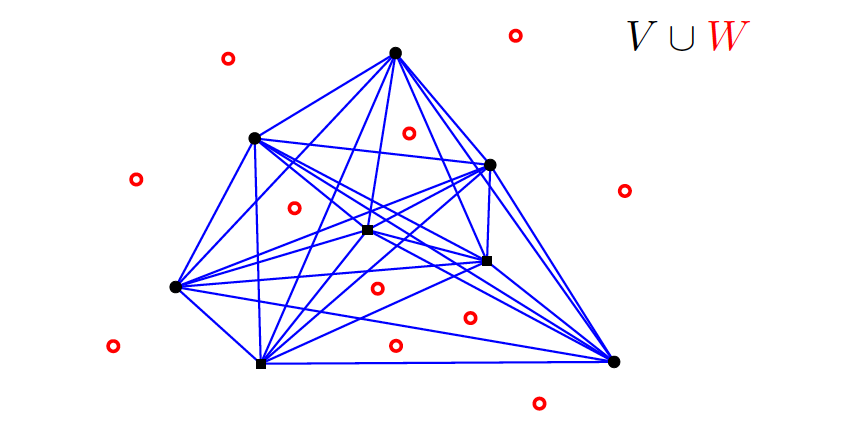
\includegraphics[keepaspectratio=true,scale=0.5]{ibagens/grafoMPRC.png}}
    \captionof{figure}{Exemplo de grafo não direcionado para V U W. Retirado do texto \cite{Washington} }
    \label{fig:GrafoVUW}
\end{minipage}

Para utilizar o algoritmos genéticos com o modelo m-PRC, o trabalho propõe dois modelos. O AGS (Algoritmo genético sequencial), que utiliza heurísticas GENIUS e 2-opt balanceada para ajustes finais para tentar melhor a solução; O AGH(Algoritmos genéticos H-1-PRC), que utiliza heurísticas H-1-PRC-MOD e 2-opt balanceada em todo o processo de resolução.

A conclusão de \cite{Washington} é que a utilização de algoritmos genéticos para a resolução de uma adaptação do problema de rotas de cobertura de veículos como bastante relevantes e de fácil manipulação. O modelo AGS resolve o problema de forma rápida e tem uma fácil implementação dentro dos critérios de comparação adotadas. O modelo AGH é mais lento e não conseguiu encontrar a solução para alguns exemplos.

Homberger, Jorg, Gehring e Hermann propuseram duas estratégias evolucionárias diferentes. As duas estratégias utilizam uma aproximação estocástica baseada na heurística das economias, ou seja, os clientes pertencentes a lista das economias são escolhidos aleatoriamente para constituir a rota. A função objetivo pondera o número de rotas, a distância total e um critério que determina a facilidade de eliminação da menor rota. 
A mutação é feita pelas heurísticas de refinamento Or-opt, 2-opt\* e $\lambda$ -Interchange. No primeiro algoritmo, o cruzamento não é executado. No segundo, o cruzamento é feito através de um procedimento uniforme. \cite{HOMBER}

O trabalho de Sabir Ribas na universidade federal de fluminense utilizou uma abordagem híbrida para resolver o Problema de Roteamento de Veículos, usando Algoritmos Genéticos com a meta-heurística Iterated Local Search e o método Variable Neighborhood Descent. Chamo de IILS-SP, desenvolvido em C++. O algoritmo foi submetido a 56 problemas teste de 100 clientes, para cada problema, executado 5 vezes em intervalos de 10min. Teve resultados melhores do que os encontrados pelo autor em sua pesquisa na literatura. \cite{SABIRRIBAS}.

Humberto,Germano e Guilherme também tentaram resolver o PRVJT utilizando GA, para a criação da população inicial utilizaram a heurística Push-Forward Insertion Heuristic. Utilizando 56 problemas de teste e 100 clientes, chamadas instâncias de Solomon de 1987, mesma base de teste utilizadas em sua revisão de literatura para comparação de resultados, utiliza a mesma metodologia de teste do Sabir Ribas. \cite{HGGUILHERME}

No trabalho de Glaydston da UniAracruz e Luiz Antônio da Instituto Nacional de Pesquisas Espaciais utilizaram algoritmos genéticos para resolver Problemas de Roteamento de Veículos Dinâmico com Janelas de Tempo, em casos reais, podem existir mudanças que podem afetar as rotas, pensando nisso, o algoritmo recalcula a rota de todos os veículos. O GA teve um resultado equivalente ou superior em alguns casos se comparado com as heurísticas. \cite{GLAYDSTON}

O trabalho de \cite{Pereira_Tavares} com uma proposta de operador de cruzamento conseguiu resultados satisfatórios no uso de GA para PRV, e propôs como trabalho futuro o uso de seu modelo para problemas especializados como o PRVJT.
